% % %
%
%	- Einleitung- 
%
%	Ziel:	Gib eine schöne Einleitung mit Motivation, Problemstellung, Zielsetzung und Struktur der Arbeit
%
%	Status: alpha
%
% % %
\chapter{Einleitung}
\label{cha:einleitung}
Die Einleitung einer Abschlussarbeit entält typischerweise eine Motivation des Themas (kein eigener Abschnitt), die Problemstellung (siehe Abschnitt \ref{sec:einleitung:problemstellung}) und die Beschreibung der Zielsetzung/des Beitrag der Arbeit (siehe Abschnitt \ref{sec:einleitung:zielsetzung}). Abschließend wird die Struktur der Arbeit vorgestellt (siehe Abschnitt \ref{sec:einleitung:struktur}).\\ %linebreak

% Beispiel Formatierungen
Hier nun ein wenig Beispieltext mit Formatierungen: \textit{Lorem ipsum dolor} sit amet, \texttt{consetetur sadipscing} elitr, sed diam \textbf{nonumy} eirmod \emph{tempor} invidunt ut labore et dolore magna aliquyam erat, sed diam voluptua. At vero eos et accusam et justo duo dolores et ea rebum. Stet clita kasd gubergren, no sea takimata sanctus est Lorem ipsum dolor sit amet. \\ %linebreak

% Beispiel Referenzierung Abbildung
Eine Abbildung wird immer erst im Text referenziert bevor sie in der Arbeit erscheint, daher siehe Abbildung \ref{fig:prozess-produkt}. \\ %linebreak

% Beispiel Referenzierung Kapitel und Abschnitte
Ganze Kapitel werden mittels Kapitel \ref{cha:einleitung} referenziert, die untergeordneten Abschnitte mittels Abschnitt \ref{sec:einleitung:problemstellung}. \\ %linebreak

% Beispiel für Referenzierung von Literatur
Aussagen, die aus der Literatur entstammen und in diesem Fall aus einem bekannten Buch für Informatiker, werden entsprechend am Ende der Satzes mit einer Referenz belegt \cite{Gamma95}. Hier noch eine Publikation von einer Konferenz als weiteres Beispiel \cite{Kolb14}

% Abbildung Prozess und Produkt - Zwei Seiten einer Medaille
\begin{figure}[htp]
\begin{center}
  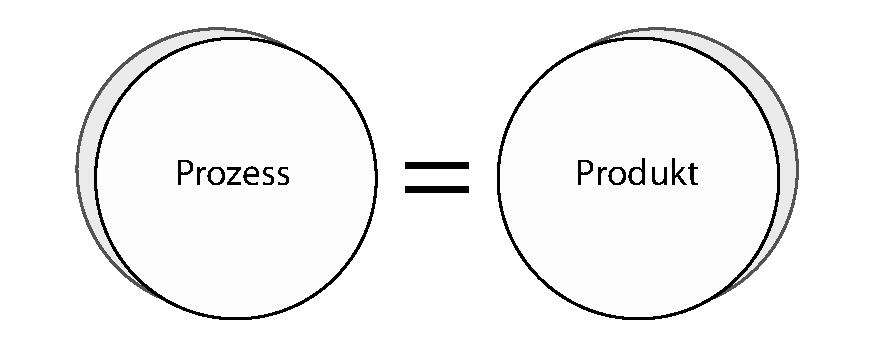
\includegraphics[width=.5\linewidth]{Prozess-und-Produkt} %pdf, jpg, png...
  \caption{Prozess und Produkt als zwei Seiten einer Medaille}
  \label{fig:prozess-produkt}
\end{center}
\end{figure}

% Abschnitt: Problemstellung
\section{Problemstellung}
\label{sec:einleitung:problemstellung}
Beschreibe in diesem Abschnitt die Problemstellung der Arbeit!

Lorem ipsum dolor sit amet, consetetur sadipscing elitr, sed diam nonumy eirmod tempor invidunt ut labore et dolore magna aliquyam erat, sed diam voluptua. At vero eos et accusam et justo duo dolores et ea rebum. Stet clita kasd gubergren, no sea takimata sanctus est Lorem ipsum dolor sit amet. 

% Abschnitt: Zielsetzung
\section{Zielsetzung}
\label{sec:einleitung:zielsetzung}
Beschreibe in diesem Abschnitt die Zielsetzung der Arbeit!

Lorem ipsum dolor sit amet, consetetur sadipscing elitr, sed diam nonumy eirmod tempor invidunt ut labore et dolore magna aliquyam erat, sed diam voluptua. At vero eos et accusam et justo duo dolores et ea rebum. Stet clita kasd gubergren, no sea takimata sanctus est Lorem ipsum dolor sit amet. 

% Abschnitt: Struktur der Arbeit
\section{Struktur der Arbeit}
\label{sec:einleitung:struktur}
Beschreibe in diesem Abschnitt die Struktur der Arbeit!

Lorem ipsum dolor sit amet, consetetur sadipscing elitr, sed diam nonumy eirmod tempor invidunt ut labore et dolore magna aliquyam erat, sed diam voluptua. At vero eos et accusam et justo duo dolores et ea rebum. Stet clita kasd gubergren, no sea takimata sanctus est Lorem ipsum dolor sit amet. 
